\documentclass{article}

\usepackage{tikz}
\usetikzlibrary{arrows,positioning} 

\renewcommand{\vec}[1]{{\textbf #1}}
\begin{document}
\section{Introduction}
\section{Methods}
\begin{enumerate}
	\item Motivation
	\begin{enumerate}
		\item Compartmental Models are a standard in disease modeling.
		\item Our model works on a general class of compartmental models.
		\item We will outline that class, then show an example on a particular influenza model.
	\end{enumerate}
	\item General
	\begin{enumerate}
		\item Class of Difference Equations Model
		\begin{enumerate}
			\item Compartmental
			\begin{enumerate}
				% \item $\vec{x}_i(t+1) = \sum_{j} \alpha_{i,j} \vec{x}_j(t) + \sum_{j,k} \alpha_{i,j,k} \vec{x}_j(t) \vec x_k(t)$
				\item $\vec{x}_i(t+1) = \sum_{j} \alpha_{i,j} \vec{x}_j(t) +  \sum_{j,k} \alpha_{i,j,k} \vec{x}_j(t) \vec x_k(t)$
				\item $\alpha_{i,j} + \alpha_{j,i} = 0$
				\item for each $k$, $\alpha_{i,j,k} + \alpha_{j,i,k} = 0$
				\item $\vec x_i(t)$ is the number of people in compartment $i$ at time $t$.
				\item sums are indexed over all compartments
				\item $\alpha_{i,j}$ represents the probability of moving from compartment $i$ to compartment $j$.
				\item $\alpha_{i,j,k}$ represents the probability that an interactions between compartment $i$ and compartment $k$ that result in a member of compartment $i$ moving to compartment $j$.
			\end{enumerate}
			\item Grouped
			\begin{enumerate}
				\item Each state follows a compartmental model
				\item Each state is determined independently
				\item Example Age cohort SIR model
			\end{enumerate}
		\end{enumerate}
		\item Agent Perspective
			\begin{enumerate}
				\item Agent Based vs Difference Equations
				\begin{enumerate}
					\item Larger Class of Models
					\item Discrete Transition Events
					\item Natural Stochastic Interpretation
				\end{enumerate}
				\item Convert Compartmental Equation into State change
				\begin{enumerate}
					\item Transform Initial Conditions - Turn a vector of counts for each state into a vector of states for each person.
					\item For each person, calculate transitions from interactions using a binomial distribution to determine conditionally infectious contacts
					\item If any of those contacts are infectious, infect that person
					\item For each person without an infectious contact, calculate transmissions not from interactions uisng using a uniform distribution
				\end{enumerate}
			\end{enumerate}
		\item Interventions
		\begin{enumerate}
			\item Interventions alter the normal behaviour of the differential equation
			\item For our purposes, interventions can cause compartment movement, or alter the probabilities of moving between compartments
			\item Computational Assumptions
			\begin{itemize}
				\item[*] Items with a $\bullet$ are necessary, but items with a $\circ$ could be relaxed at the expense of either writing more code, or using more time/space.
				\item All Interventions either change people from one state to another or reduce some $\alpha$..
				\item[$\circ$] People that are have their state changed due to intervention will not change state again.
				\item[$\circ$] We assume interventions only reduce $\alpha$.
				\item[$\circ$] We assume that interventions only target $\alpha_{i,j,k}$ rather than $\alpha_{i,j}$.
			\end{itemize}
			\item Move between compartments
			\begin{enumerate}
				\item Vaccination
				\item Quarantine
				\item Treatment
				\item function that modifies the states of every person based on that vector, time, and intervention parameters.
			\end{enumerate}
			\item Alter probabilities
			\begin{enumerate}
				\item Social Distancing
				\item Hygiene
				\item Vaccination that isn't fully innoculating
				\item function that depends on time, state transition from, state transition to, state interacted with, and the ranodm number
			\end{enumerate}
		\end{enumerate}
	\end{enumerate}
	\item Specific
	\begin{enumerate}
		\item Influenza Example Model
		\begin{enumerate}
			\item SIR(S) model
			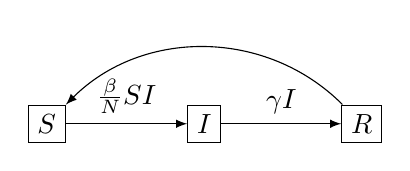
\begin{tikzpicture}
				\draw (0,0) node[draw=black] (S) {$S$};
				\draw (2,0) node[draw=black] (I) {$I$};
				\draw (4,0) node[draw=black] (R) {$R$};
				
				\draw[-latex] (S) -> (I) node[midway,above] {$\frac{\beta}{N} S I$};
				\draw[-latex] (I) -> (R) node[midway,above] {$\gamma I$};
				\draw[-latex] (R) to[out=135,in=45] (S);
			\end{tikzpicture}
			\item $N$ is the total population.
			\item $\beta$ is the transmission coefficient
			\item $\gamma$ is the recovery rate
			\item We can ignore $R\rightarrow S$, because by estimating over a single season.
			\item Talia said to check Sarah Cobey and Marc Lipschitz work for parameters
		\end{enumerate}
		\item Particular Interventions
		\begin{enumerate}
			\item Vaccination
			\begin{enumerate}
				\item Description of Intervention
				\item Implementation in Model
			\end{enumerate}
			\item Treatment
			\begin{enumerate}
				\item Description of Intervention
				\item Implementation in Model
			\end{enumerate}
			\item Social Distancing/Hygiene
			\begin{enumerate}
				\item Description of Intervention
				\item Implementation in Model
			\end{enumerate}
			\item None
			\begin{enumerate}
				\item Description of Intervention
				\item Implementation in Model
			\end{enumerate}
		\end{enumerate}
	\end{enumerate}
\end{enumerate}
\section{Results}
\section{Discussion}

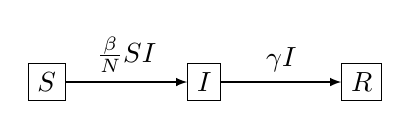
\begin{tikzpicture}
\draw (0,0) node[draw=black] (S) {$S$};
\draw (2,0) node[draw=black] (I) {$I$};
\draw (4,0) node[draw=black] (R) {$R$};

\draw[-latex] (S) -> (I) node[midway,above] {$\frac{\beta}{N} S I$};
\draw[-latex] (I) -> (R) node[midway,above] {$\gamma I$};

\end{tikzpicture}

\bibliography{bib}{}
\bibliographystyle{plain}
\end{document}

% Don't use agent based modeling